\section{Casi d'uso}
\subsection{Introduzione}
In questa sezione del documento vengono analizzati nel dettaglio i casi d'uso individuati per il sistema.
nel corso dell'analisi del \href{https://7last.github.io/docs/rtb/documentazione-interna/glossario\#capitolato}{capitolato\textsubscript{G}} e dei colloqui con la proponente.

\subsection{Struttura dei casi d'uso}
In tutto il documento ci si riferirà ai casi d'uso utilizzando la sigla \texttt{UC} seguita dal rispettivo codice nella forma
\begin{center}
	\textbf{UC-[identificativo\_caso\_principale].[identificativo\_sotto\_caso]}
\end{center}

il quale permette di utilizzarlo come riferimento in questo e altri documenti.\\
Per ciascun caso d'uso vengono definiti i seguenti elementi:
\begin{itemize}
	\item \textbf{Attore principale}: l'attore primariamente coinvolto nel caso d'uso;
	\item \textbf{Precondizioni}: le condizioni che devono essere verificate affinché il caso d'uso possa essere
	      eseguito;
	\item \textbf{Postcondizioni}: le condizioni che devono essere verificate al termine dell'esecuzione del caso
	\item \textbf{Scenario principale}: la sequenza di passi che descrive il comportamento del sistema durante
	      l'esecuzione del caso d'uso;
	\item \href{https://7last.github.io/docs/rtb/documentazione-interna/glossario\#user-story}{\textbf{User story}\textsubscript{G}} (opzionale): una descrizione testuale del caso d'uso;
\end{itemize}


\subsection{Attori}
I seguenti attori sono coinvolti nei casi d'uso:
\begin{itemize}
	\item Impiegati presso \textbf{autorità locali}: essi possono accedere al sistema per visualizzare i dati
	      monitoraggio della \textit{Smart City}.
	\item \textbf{Sensori}: sorgente di dati con un determinato dominio di interesse che effettua misurazioni
	      e trasmette i dati al sistema.
\end{itemize}

\subsection{Elenco dei casi d'uso}
\subsubsection{UC-1: Visualizzazione dashboard generale}
\begin{center}
	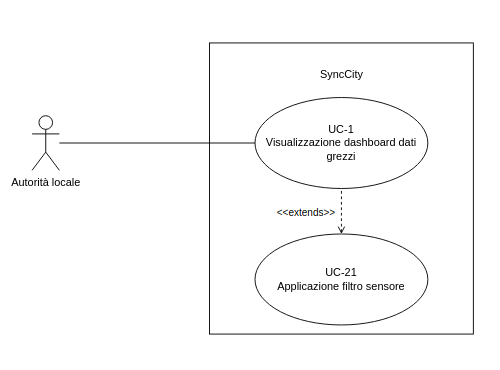
\includegraphics[width=0.6\textwidth]{analisi_dei_requisiti/UC-1.png}
	\captionof{figure}{UC-1: Visualizzazione \href{https://7last.github.io/docs/rtb/documentazione-interna/glossario#dashboard}{dashboard\textsubscript{G}} generale}
\end{center}
\subsubsubsection{UC-1.1: Visualizzazione mappa interattiva sensori}
\begin{center}
	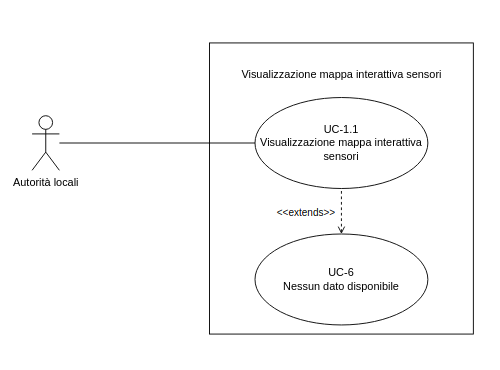
\includegraphics[width=0.6\textwidth]{analisi_dei_requisiti/UC-1.1.png}
	\captionof{figure}{UC-1.1: Visualizzazione mappa interattiva sensori}
\end{center}
\subsubsubsection{UC-1.2: Visualizzazione tabella sensori}
\begin{center}
	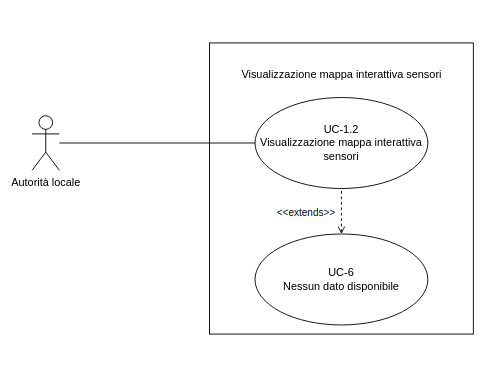
\includegraphics[width=0.6\textwidth]{analisi_dei_requisiti/UC-1.2.png}
	\captionof{figure}{UC-1.2: Visualizzazione tabella sensori}
\end{center}

\subsubsection{UC-2: Visualizzazione dashboard dati atmosferici}
\begin{center}
	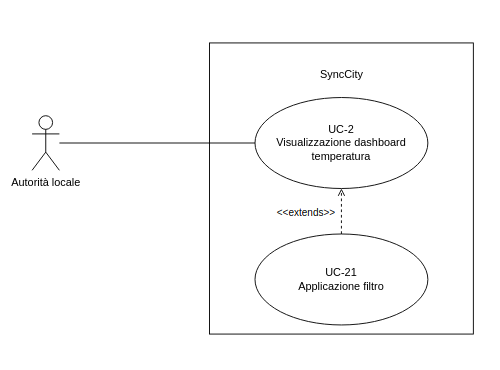
\includegraphics[width=0.6\textwidth]{analisi_dei_requisiti/UC-2.png}
	\captionof{figure}{UC-2: Visualizzazione \href{https://7last.github.io/docs/rtb/documentazione-interna/glossario#dashboard}{dashboard\textsubscript{G}} dati atmosferici}
\end{center}

% temperatura
\subsubsubsection{UC-2.1: Visualizzazione grafico time series per temperatura}
\begin{center}
	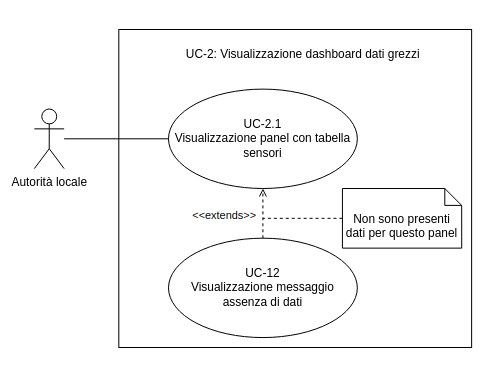
\includegraphics[width=0.75\textwidth]{analisi_dei_requisiti/UC-2.1.png}
	\captionof{figure}{UC-2.1: Visualizzazione grafico time series per temperatura}
\end{center}
\subsubsubsection{UC-2.2: Visualizzazione \textit{panel} temperatura in tempo reale}
\begin{center}
	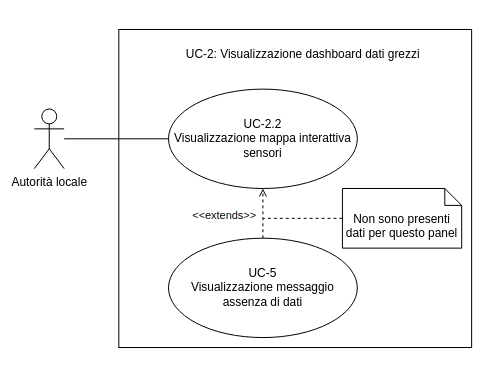
\includegraphics[width=0.75\textwidth]{analisi_dei_requisiti/UC-2.2.png}
	\captionof{figure}{UC-2.2: Visualizzazione \textit{panel} temperatura in tempo reale}
\end{center}

\subsubsubsection{UC-2.3: Visualizzazione \textit{panel} temperatura media}
\begin{center}
	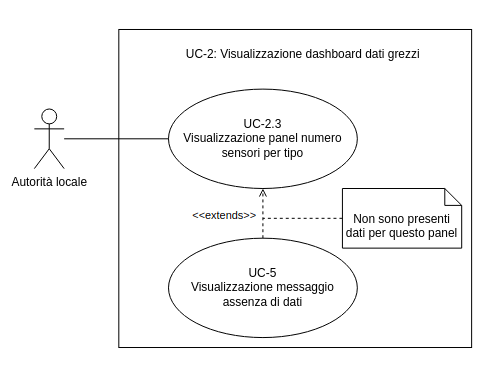
\includegraphics[width=0.75\textwidth]{analisi_dei_requisiti/UC-2.3.png}
	\captionof{figure}{UC-2.3: Visualizzazione \textit{panel} temperatura media}
\end{center}
\subsubsubsection{UC-2.4: Visualizzazione \textit{panel} temperatura massima}
\begin{center}
	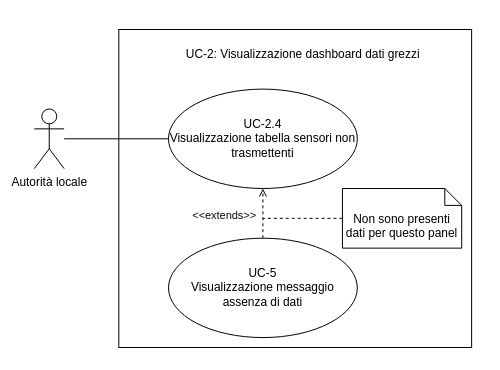
\includegraphics[width=0.75\textwidth]{analisi_dei_requisiti/UC-2.4.png}
	\captionof{figure}{UC-2.4: Visualizzazione \textit{panel} temperatura massima}
\end{center}
\subsubsubsection{UC-2.5: Visualizzazione \textit{panel} temperatura minima}
\begin{center}
	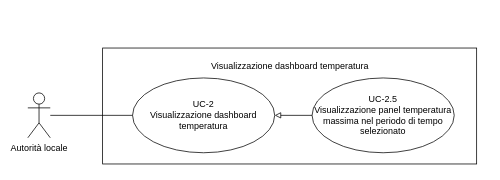
\includegraphics[width=0.75\textwidth]{analisi_dei_requisiti/UC-2.5.png}
	\captionof{figure}{UC-2.5: Visualizzazione \textit{panel} temperatura minima}
\end{center}

% umidità
\subsubsubsection{UC-2.6: Visualizzazione grafico time series per umidità}
\begin{center}
	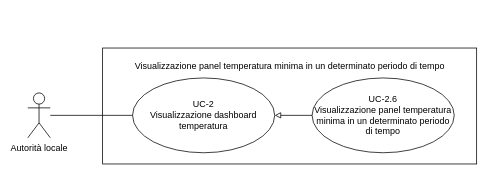
\includegraphics[width=0.75\textwidth]{analisi_dei_requisiti/UC-2.6.png}
	\captionof{figure}{UC-2.6: Visualizzazione grafico time series per umidità}
\end{center}

\subsubsubsection{UC-2.7: Visualizzazione \textit{panel} umidità in tempo reale}
\begin{center}
	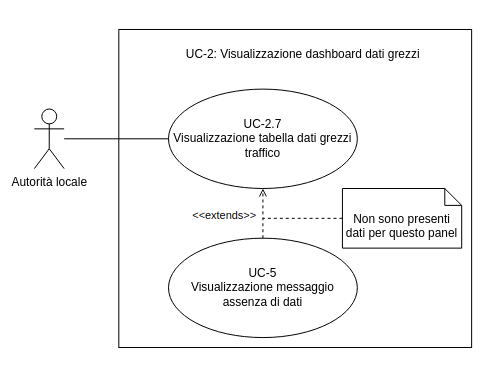
\includegraphics[width=0.75\textwidth]{analisi_dei_requisiti/UC-2.7.png}
	\captionof{figure}{UC-2.7: Visualizzazione \textit{panel} umidità in tempo reale}
\end{center}

\subsubsubsection{UC-2.8: Visualizzazione \textit{panel} umidità media}
\begin{center}
	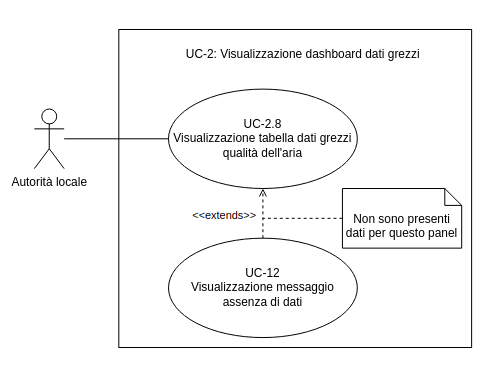
\includegraphics[width=0.75\textwidth]{analisi_dei_requisiti/UC-2.8.png}
	\captionof{figure}{UC-2.8: Visualizzazione \textit{panel} umidità media}
\end{center}

\subsubsubsection{UC-2.9: Visualizzazione \textit{panel} umidità massima}
\begin{center}
	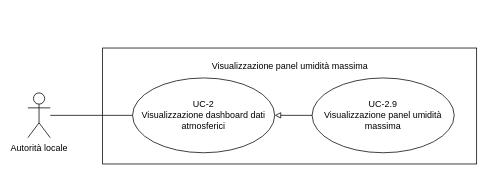
\includegraphics[width=0.75\textwidth]{analisi_dei_requisiti/UC-2.9.png}
	\captionof{figure}{UC-2.9: Visualizzazione \textit{panel} umidità massima}
\end{center}

\subsubsubsection{UC-2.10: Visualizzazione \textit{panel} umidità minima}
\begin{center}
	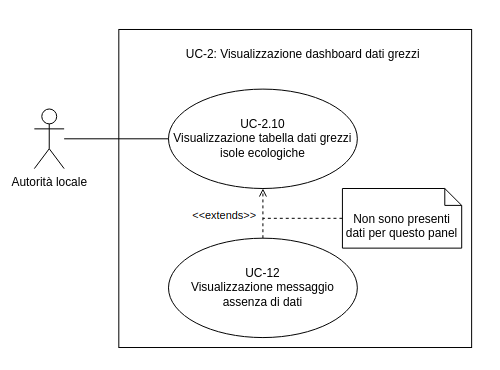
\includegraphics[width=0.75\textwidth]{analisi_dei_requisiti/UC-2.10.png}
	\captionof{figure}{UC-2.10: Visualizzazione \textit{panel} umidità minima}
\end{center}

% pressione
\subsubsubsection{UC-2.11: Visualizzazione grafico time series per pressione}
\begin{center}
	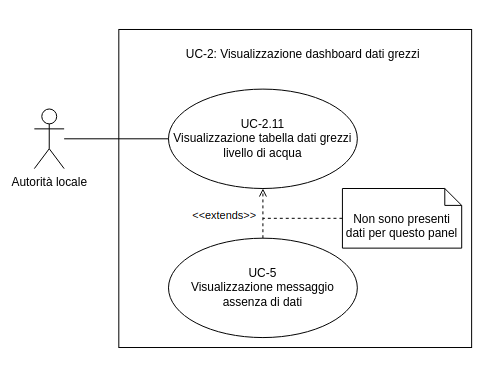
\includegraphics[width=0.75\textwidth]{analisi_dei_requisiti/UC-2.11.png}
	\captionof{figure}{UC-2.11: Visualizzazione grafico time series per pressione}
\end{center}
\subsubsubsection{UC-2.12: Visualizzazione \textit{panel} pressione in tempo reale}
\begin{center}
	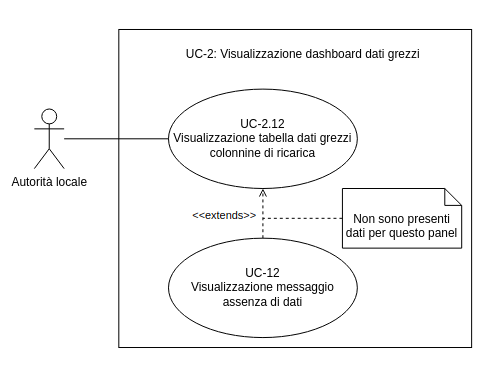
\includegraphics[width=0.75\textwidth]{analisi_dei_requisiti/UC-2.12.png}
	\captionof{figure}{UC-2.12: Visualizzazione \textit{panel} pressione in tempo reale}
\end{center}
\subsubsubsection{UC-2.13: Visualizzazione \textit{panel} pressione media}
\begin{center}
	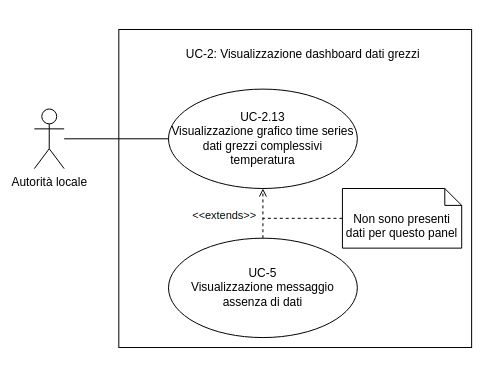
\includegraphics[width=0.75\textwidth]{analisi_dei_requisiti/UC-2.13.png}
	\captionof{figure}{UC-2.13: Visualizzazione \textit{panel} pressione media}
\end{center}
\subsubsubsection{UC-2.14: Visualizzazione \textit{panel} pressione massima}
\begin{center}
	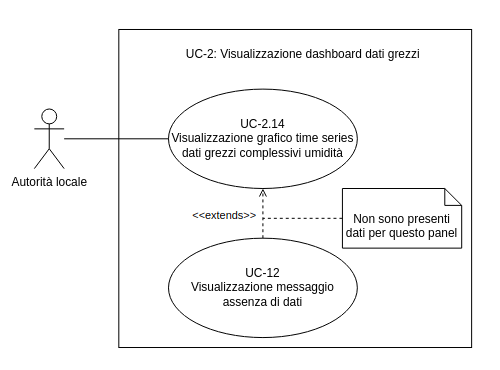
\includegraphics[width=0.75\textwidth]{analisi_dei_requisiti/UC-2.14.png}
	\captionof{figure}{UC-2.14: Visualizzazione \textit{panel} pressione massima}
\end{center}
\subsubsubsection{UC-2.15: Visualizzazione \textit{panel} pressione minima}
\begin{center}
	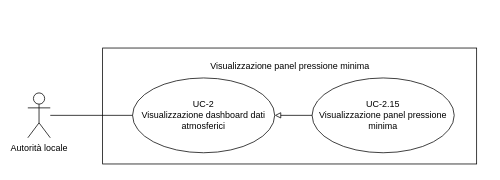
\includegraphics[width=0.75\textwidth]{analisi_dei_requisiti/UC-2.15.png}
	\captionof{figure}{UC-2.15: Visualizzazione \textit{panel} pressione minima}
\end{center}

% precipitazioni
\subsubsubsection{UC-2.16: Visualizzazione grafico time series per quantità di precipitazioni}
\begin{center}
	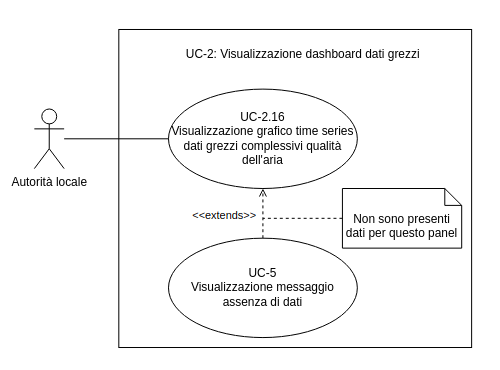
\includegraphics[width=0.75\textwidth]{analisi_dei_requisiti/UC-2.16.png}
	\captionof{figure}{UC-2.16: Visualizzazione grafico time series per precipitazioni}
\end{center}

\subsubsubsection{UC-2.17: Visualizzazione \textit{panel} quantità di precipitazioni in tempo reale}
\subsubsubsection{UC-2.18: Visualizzazione \textit{panel} quantità totale di precipitazioni}
\begin{center}
	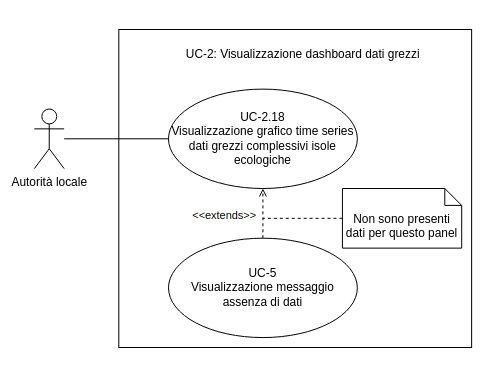
\includegraphics[width=0.75\textwidth]{analisi_dei_requisiti/UC-2.18.png}
	\captionof{figure}{UC-2.18: Visualizzazione \textit{panel} quantità totale di precipitazioni}
\end{center}

\subsubsubsection{UC-2.19: Visualizzazione \textit{panel} quantità media di precipitazioni}
\begin{center}
	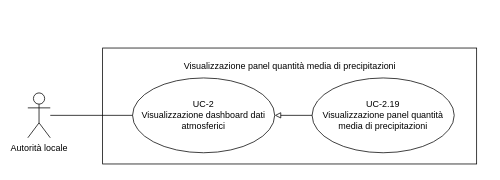
\includegraphics[width=0.75\textwidth]{analisi_dei_requisiti/UC-2.19.png}
	\captionof{figure}{UC-2.19: Visualizzazione \textit{panel} quantità media di precipitazioni}
\end{center}

% polveri sottili
\subsubsubsection{UC-2.20: Visualizzazione grafico time series per polveri sottili nell'aria}
\begin{center}
	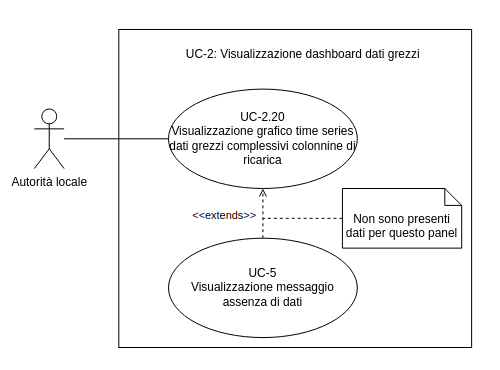
\includegraphics[width=0.75\textwidth]{analisi_dei_requisiti/UC-2.20.png}
	\captionof{figure}{UC-2.20: Visualizzazione grafico time series per polveri sottili nell'aria}
\end{center}

\subsubsubsection{UC-2.21: Visualizzazione \textit{panel} polveri sottili nell'aria in tempo reale}
\begin{center}
	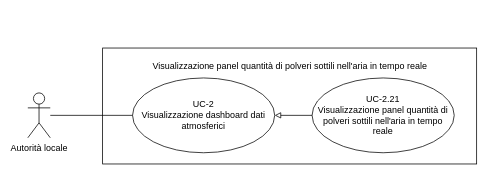
\includegraphics[width=0.75\textwidth]{analisi_dei_requisiti/UC-2.21.png}
	\captionof{figure}{UC-2.21: Visualizzazione \textit{panel} polveri sottili nell'aria in tempo reale}
\end{center}

\subsubsubsection{UC-2.22: Visualizzazione \textit{panel} giorno con maggiore concentrazione di polveri sottili}
\begin{center}
	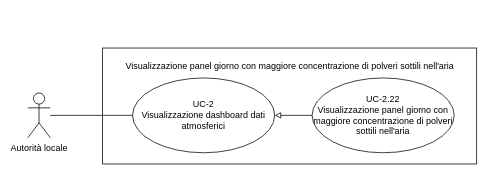
\includegraphics[width=0.75\textwidth]{analisi_dei_requisiti/UC-2.22.png}
	\captionof{figure}{UC-2.22: Visualizzazione \textit{panel} giorno con maggiore concentrazione di polveri sottili}
\end{center}

\subsubsubsection{UC-2.23: Visualizzazione \textit{panel} giorno con minore concentrazione di polveri sottili}
\begin{center}
	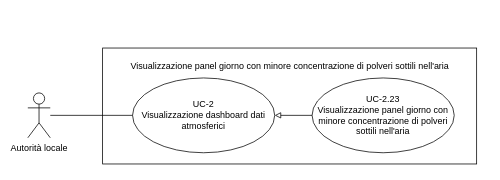
\includegraphics[width=0.75\textwidth]{analisi_dei_requisiti/UC-2.23.png}
	\captionof{figure}{UC-2.23: Visualizzazione \textit{panel} giorno con minore concentrazione di polveri sottili}
\end{center}

\subsubsubsection{UC-2.24: Visualizzazione \textit{panel} media di polveri sottili nell'aria}
\begin{center}
	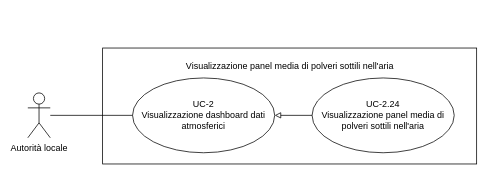
\includegraphics[width=0.75\textwidth]{analisi_dei_requisiti/UC-2.24.png}
	\captionof{figure}{UC-2.24: Visualizzazione \textit{panel} media di polveri sottili nell'aria}
\end{center}

\subsubsection{UC-3: Visualizzazione dashboard dati urbani}
\begin{center}
	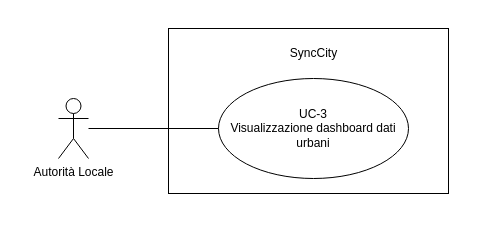
\includegraphics[width=0.6\textwidth]{analisi_dei_requisiti/UC-3.png}
\end{center}
\subsubsubsection{UC-3.1: Visualizzazione dati traffico}
\subsubsubsubsection{UC-3.1.1: Visualizzazione grafico time series per traffico giornaliero}

\subsubsubsection{UC-3.2: Visualizzazione dati lavori in corso}
\subsubsubsubsection{UC-3.2.1: Visualizzazione mappa interattiva lavori in corso}

\subsubsubsection{UC-3.3: Visualizzazione dati incidenti}
\subsubsubsubsection{UC-3.3.1: Visualizzazione grafico time series per incidenti}
\subsubsubsubsection{UC-3.3.2: Visualizzazione mappa interattiva incidenti in tempo reale}
\subsubsubsubsection{UC-3.3.3: Visualizzazione \textit{panel} incidenti nell'ultimo mese}
\subsubsubsubsection{UC-3.3.4: Visualizzazione \textit{panel} incidenti nell'ultimo anno}

\subsubsubsection{UC-3.4: Visualizzazione dati colonnine di ricarica}
\subsubsubsubsection{UC-3.4.1: Visualizzazione mappa interattiva colonnine di ricarica con stato di funzionamento}
\subsubsubsubsection{UC-3.4.2: Visualizzazione \textit{panel} con conteggio colonnine guaste e funzionanti}

\subsubsubsection{UC-3.5: Visualizzazione dati isole ecologiche}
\subsubsubsubsection{UC-3.5.1: Visualizzazione mappa interattiva isole ecologiche con stato di riempimento}
\subsubsubsubsection{UC-3.5.2: Visualizzazione \textit{panel} con conteggio isole piene}

\subsubsubsection{UC-3.6: Visualizzazione dati parcheggi}
\subsubsubsubsection{UC-3.6.1: Visualizzazione mappa interattiva parcheggi con rispettivo stato di occupazione}
\subsubsubsubsection{UC-3.6.2: Visualizzazione \textit{panel} con conteggio parcheggi occupati e liberi}

\subsubsubsection{UC-3.7: Visualizzazione dati livello di acqua}
\subsubsubsubsection{UC-3.7.1: Visualizzazione grafico time series per livello di acqua}

\subsubsection{UC-4: Visualizzazione allerte}

\subsubsection{UC-5: Visualizzazione con filtri}

\subsubsection{UC-6: Nessun dato disponibile}

\subsubsection{UC-7: Trasmissione dati temperatura}

\subsubsection{UC-8: Trasmissione dati umidità}

\subsubsection{UC-9: Trasmissione dati pressione}

\subsubsection{UC-10: Trasmissione dati vento}

\subsubsection{UC-11: Trasmissione dati precipitazioni}

\subsubsection{UC-12: Trasmissione dati polveri sottili}

\subsubsection{UC-13: Trasmissione dati traffico}

\subsubsection{UC-14: Trasmissione dati lavori in corso}

\subsubsection{UC-15: Trasmissione dati incidenti}

\subsubsection{UC-16: Trasmissione dati colonnine di ricarica}

\subsubsection{UC-17: Trasmissione dati isole ecologiche}

\subsubsection{UC-18: Trasmissione dati parcheggi}

\subsubsection{UC-19: Trasmissione dati livello di acqua}


















